\documentclass{article}
\usepackage{cmap}
\usepackage[utf8]{inputenc}
\usepackage[english,ukrainian]{babel}
\usepackage{graphicx}
\usepackage{geometry}
\usepackage{listings}
\usepackage{amsmath}
\usepackage{float}
\geometry{
	a4paper,
	left=20mm,
	right=20mm,
	top=20mm,
	bottom=20mm
}
\lstset{
	language=c++,
	tabsize=4,
	keepspaces,
	showstringspaces=false,
	breaklines,
}
\graphicspath{ {./pictures} }
\setlength{\parindent}{4em}

\newcommand\subject{Операційні системи}
\newcommand\lecturer{старший викладач кафедри ПЗ\\Грицай О.Д.}
\newcommand\teacher{старший викладач кафедри ПЗ\\Грицай О.Д.}
\newcommand\mygroup{ПЗ-22}
\newcommand\lab{7}
\newcommand\theme{Статичні та динамічні бібліотеки. WINDOWS та LINUX}
\newcommand\purpose{Ознайомитися з статичними та динамічними бібліотеками в операційних
	системах WINDOWS та LINUX. Навчитися реалізовувати статичні та динамічні
	бібліотеки}

\begin{document}
\begin{normalsize}
	\begin{titlepage}
		\thispagestyle{empty}
		\begin{center}
			\textbf{МІНІСТЕРСТВО ОСВІТИ І НАУКИ УКРАЇНИ\\
				НАЦІОНАЛЬНИЙ УНІВЕРСИТЕТ "ЛЬВІВСЬКА ПОЛІТЕХНІКА"}
		\end{center}
		\begin{flushright}
			Інститут \textbf{КНІТ}\\
			Кафедра \textbf{ПЗ}
		\end{flushright}
		\vspace{200pt}
		\begin{center}
			\textbf{ЗВІТ}\\
			\vspace{10pt}
			До лабораторної роботи № \lab\\
			\textbf{На тему}: “\textit{\theme}”\\
			\textbf{З дисципліни}: “\subject”
		\end{center}
		\vspace{112pt}
		\begin{flushright}
			
			\textbf{Лектор}:\\
			\lecturer\\
			\vspace{28pt}
			\textbf{Виконав}:\\
			
			студент групи \mygroup\\
			Коваленко Д.М.\\
			\vspace{28pt}
			\textbf{Прийняла}:\\
			
			\teacher\\
			
			\vspace{28pt}
			«\rule{1cm}{0.15mm}» \rule{1.5cm}{0.15mm} 2022 р.\\
			$\sum$ = \rule{1cm}{0.15mm}……………\\
			
		\end{flushright}
		\vspace{\fill}
		\begin{center}
			\textbf{Львів — 2022}
		\end{center}
	\end{titlepage}
		
	\begin{description}
		\item[Тема.] \theme.
		\item[Мета.] \purpose.
	\end{description}

	\section*{Лабораторне завдання}
	
	\begin{figure}[H]
		\centering
		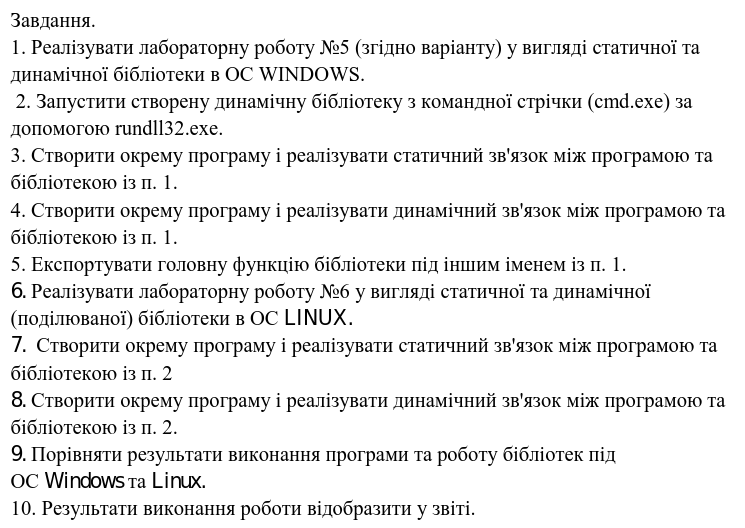
\includegraphics[scale=0.7]{v}
	\end{figure}
	\begin{center}
		2. Обчислити суму елементів заданого масиву (кількість елементів >10000,
		елементи рандомні) (Синхронізація: семафор, спінблокувавння)
	\end{center}

	\section*{Хід роботи}	
	\section*{WINDOWS}
	\textbf{main.cpp}
	\begin{lstlisting}
#include <iostream>
#include <Windows.h>
#include "libSum.h"
#ifndef RUNTIME
#include "dllSum.h"
#else
typedef int(__cdecl* DLLSUMUP)(int*, int);
#endif

int main() {
	int len;
	std::cout << "Enter array len: ";
	std::cin >> len;
	int* arr = new int[len];
	std::srand(static_cast<unsigned int>(std::time(nullptr)));
	for (int i = 0; i < len; i++) arr[i] = rand() % 10;
	
	int sum = libSumUp(arr, len);
	std::cout << "Sum from static lib: " << sum << std::endl;
	
	#ifndef RUNTIME
	int dllSum = dllSumUp(arr, len);
	std::cout << "Sum from dynamic lib (using load-time linking): " << dllSum << std::endl;
	#else
	HINSTANCE hinstLib;
	DLLSUMUP dllSumUp;
	BOOL fFreeResult, fRunTimeLinkSuccess = FALSE;
	
	hinstLib = LoadLibrary(TEXT("dllSum.dll"));
	
	if (hinstLib != NULL) {
		dllSumUp = (DLLSUMUP)GetProcAddress(hinstLib, "dllSumUp");
		
		if (NULL != dllSumUp) {
			fRunTimeLinkSuccess = TRUE;
			int dllSum = (dllSumUp)(arr, len);
			std::cout << "Sum from dynamic lib (using run-time linking): " << dllSum << std::endl;
		}
		
		fFreeResult = FreeLibrary(hinstLib);
	}
	
	if (!fRunTimeLinkSuccess)
	std::cout << "Failed to link on runtime" << std::endl;
	#endif
}

	\end{lstlisting}
	
	\noindent\textbf{libSum.h}
	\begin{lstlisting}
#pragma once
namespace sum {
	int sumUp(int* arr, int len);
}
		
	\end{lstlisting}

	\noindent\textbf{libSum.cpp}
	\begin{lstlisting}
#include "pch.h"
#include "framework.h"
#include "libSum.h"

namespace sum {
	int sumUp(int* arr, int len) {
		int sum = 0;
		for (int i = 0; i < len; i++) sum += arr[i];
		return sum;
	}
}
		
	\end{lstlisting}
	
	\noindent\textbf{dllSum.h}
	\begin{lstlisting}
#pragma once

#ifndef DLLSUM_EXPORTS
#define DLLSUM_API __declspec(dllexport)
#else
#define DLLSUM_API __declspec(dllimport)
#endif

extern "C" DLLSUM_API int dllSumUp(int* arr, int len);
		
	\end{lstlisting}
		
	\noindent\textbf{dllSum.cpp}
	\begin{lstlisting}
#include "pch.h"
#include "dllSum.h"

int dllSumUp(int* arr, int len) {
	int sum = 0;
	for (int i = 0; i < len; i++) sum += arr[i];
	return sum;
}
		
	\end{lstlisting}
	
	\begin{figure}[H]
		\centering
		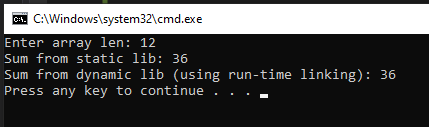
\includegraphics[scale=0.9]{1}
		\caption{Виконання програми (динамічний зв'язок з динамічною бібліотекою)}
	\end{figure}

	\begin{figure}[H]
		\centering
		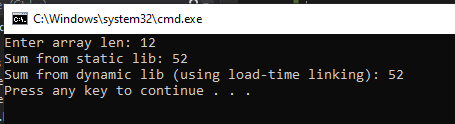
\includegraphics[scale=0.85]{2}
		\caption{Виконання програми (статичний зв'язок з динамічною бібліотекою)}
	\end{figure}

	\section*{LINUX}
	\textbf{aSum.h}
	\begin{lstlisting}
extern "C" int soSumUp(int* arr, int len);	
	\end{lstlisting}
	
	\noindent\textbf{aSum.cpp}
	\begin{lstlisting}
#include "aSum.h"

int sumUp(int* arr, int len) {
	int sum = 0;
	for (int i = 0; i < len; i++) sum += arr[i];
	return sum;
}

	\end{lstlisting}
	
	\noindent\textbf{soSum.h}
	\begin{lstlisting}
int soSumUp(int* arr, int len);
		
	\end{lstlisting}
	
	\noindent\textbf{soSum.cpp}
	\begin{lstlisting}
#include "soSum.h"

int soSumUp(int* arr, int len) {
	int sum = 0;
	for (int i = 0; i < len; i++) sum += arr[i];
	return sum;
}

	\end{lstlisting}
	
	\noindent\textbf{main.cpp}
	\begin{lstlisting}
#include <iostream>
#include "aSum.h"
#define RUNTIME
#ifndef RUNTIME
#include "soSum.h"
#else
#include <dlfcn.h>
int (*soSumUp)(int*, int);
#endif

int main() {
	int len;
	std::cout << "Enter array len: ";
	std::cin >> len;
	int* arr = new int[len];
	srand(static_cast<unsigned int>(time(nullptr)));
	for (int i = 0; i < len; i++) arr[i] = rand() % 10;
	
	int aSum = sumUp(arr, len);
	std::cout << "Sum from static lib: " << aSum << std::endl;
	
#ifndef RUNTIME
	int soSum = soSumUp(arr, len);
	std::cout << "Sum from dynamic lib (using load-time linking: " << soSum << std::endl;
#else
	void* lib;
	lib = dlopen("./libSum.so", RTLD_LAZY);
	if (!lib)
		std::cout << "Failed to link on runtime" << std::endl;
	
	soSumUp = (int (*)(int*, int))dlsym(lib, "soSumUp");
	
	int soSum = (*soSumUp)(arr, len);
	std::cout << "Sum from dynamic lib (using run-time linking: " << soSum << std::endl;
	
	dlclose(lib);
#endif
}

	\end{lstlisting}
	
	\noindent\textbf{run.sh}
	\begin{lstlisting}
#!/bin/sh
export LD_LIBRARY_PATH=.

g++ -c main.cpp
g++ -c aSum.cpp
ar rc libSum.a aSum.o
ranlib libSum.a
g++ -fPIC -c soSum.cpp
g++ -shared -o libSum.so soSum.o
g++ main.o libSum.a libSum.so
./a.out

rm *.a *.o *.so *.out
		
	\end{lstlisting}
	
		\begin{figure}[H]
		\centering
		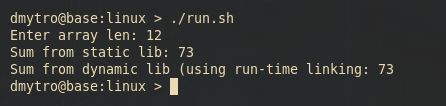
\includegraphics[scale=0.9]{4}
		\caption{Виконання програми (динамічний зв'язок з динамічною бібліотекою)}
	\end{figure}

	\begin{figure}[H]
	\centering
	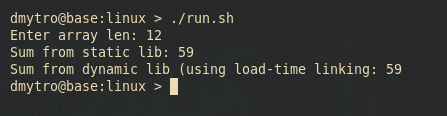
\includegraphics[scale=0.9]{5}
	\caption{Виконання програми (статичний зв'язок з динамічною бібліотекою)}
	\end{figure}
	
	\section*{Висновок}
	Під час виконання лабораторної роботи я ознайомився з статичними та динамічними бібліотеками в операційних
	системах WINDOWS та LINUX. Навчився реалізовувати статичні та динамічні
	бібліотеки
	
	 
\end{normalsize}
\end{document}
